\documentclass[12pt,letterpaper]{article}
\usepackage{graphicx,textcomp}
\usepackage{natbib}
\usepackage{setspace}
\usepackage{fullpage}
\usepackage{color}
\usepackage[reqno]{amsmath}
\usepackage{amsthm}
\usepackage{fancyvrb}
\usepackage{amssymb,enumerate}
\usepackage[all]{xy}
\usepackage{endnotes}
\usepackage{lscape}
\newtheorem{com}{Comment}
\usepackage{float}
\usepackage{hyperref}
\newtheorem{lem} {Lemma}
\newtheorem{prop}{Proposition}
\newtheorem{thm}{Theorem}
\newtheorem{defn}{Definition}
\newtheorem{cor}{Corollary}
\newtheorem{obs}{Observation}
\usepackage[compact]{titlesec}
\usepackage{dcolumn}
\usepackage{tikz}
\usetikzlibrary{arrows}
\usepackage{multirow}
\usepackage{xcolor}
\newcolumntype{.}{D{.}{.}{-1}}
\newcolumntype{d}[1]{D{.}{.}{#1}}
\definecolor{light-gray}{gray}{0.65}
\usepackage{url}
\usepackage{listings}
\usepackage{color}

\definecolor{codegreen}{rgb}{0,0.6,0}
\definecolor{codegray}{rgb}{0.5,0.5,0.5}
\definecolor{codepurple}{rgb}{0.58,0,0.82}
\definecolor{backcolour}{rgb}{0.95,0.95,0.92}

\lstdefinestyle{mystyle}{
	backgroundcolor=\color{backcolour},   
	commentstyle=\color{codegreen},
	keywordstyle=\color{magenta},
	numberstyle=\tiny\color{codegray},
	stringstyle=\color{codepurple},
	basicstyle=\footnotesize,
	breakatwhitespace=false,         
	breaklines=true,                 
	captionpos=b,                    
	keepspaces=true,                 
	numbers=left,                    
	numbersep=5pt,                  
	showspaces=false,                
	showstringspaces=false,
	showtabs=false,                  
	tabsize=2
}
\lstset{style=mystyle}
\newcommand{\Sref}[1]{Section~\ref{#1}}
\newtheorem{hyp}{Hypothesis}

\title{Problem Set 5}
\date{Due: March 4, 2020}
\author{QTM 200: Applied Regression Analysis}

\begin{document}
	\maketitle
	
	\section*{Instructions}
	\begin{itemize}
		\item Please show your work! You may lose points by simply writing in the answer. If the problem requires you to execute commands in \texttt{R}, please include the code you used to get your answers. Please also include the \texttt{.R} file that contains your code. If you are not sure if work needs to be shown for a particular problem, please ask.
		\item Your homework should be submitted electronically on the course GitHub page in \texttt{.pdf} form.
		\item This problem set is due at the beginning of class on Wednesday, March 4, 2020. No late assignments will be accepted.
		\item Total available points for this homework is 100.
	\end{itemize}
	
		\vspace{.5cm}
	
\noindent  Using the \texttt{teengamb} dataset, fit a model with \texttt{gamble} as the response and the other variables as predictors. 

\vspace{.5cm}
\lstinputlisting[language=R, firstline=41, lastline=43]{Alice-PS5.R}  
\vspace{.5cm}
Answer the following questions:
\vspace{.5cm}
\begin{enumerate}[(a)]
	 \item Check the constant variance assumption for the errors by plotting the residuals versus the fitted values. 
	 
	 \lstinputlisting[language=R, firstline=45, lastline=47]{Alice-PS5.R}
  
	\begin{figure}[h!]\centering
	 	\label{top}
	 	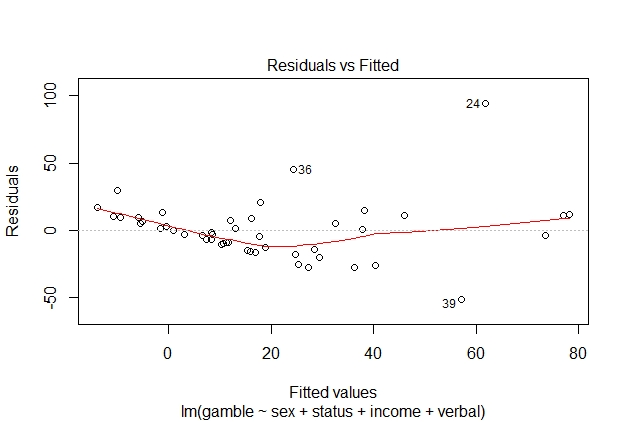
\includegraphics[width=.75\textwidth]{Regressionplot1.JPEG}
	 	\caption{The residual distribution is not very uniform, with variance growing larger for larger fitted values. We therefore cannot safely assume equal variance}
 	\end{figure}
\newpage 
	\item Check the normality assumption with a Q-Q plot of the studentized residuals.	
	
	\begin{figure}[h!]\centering
		\label{bottom}
		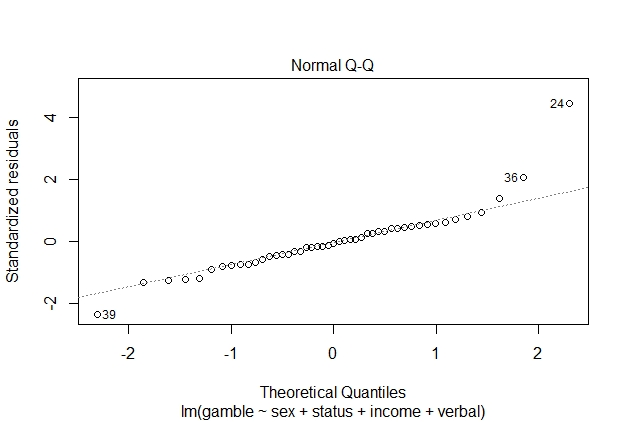
\includegraphics[width=.75\textwidth]{Regressionplot2.JPEG}
		\caption{The Q-Q plot for standardized residuals is roughly linear, we can therefore infer that the distributions of all the variables are approximately normal.}
	\end{figure}
	
	\item Check for large leverage points by plotting the $h$ values.
	\lstinputlisting[language=R, firstline=48, lastline=53]{Alice-PS5.R}
		
	\begin{figure}[h!]\centering
	\label{hat}
	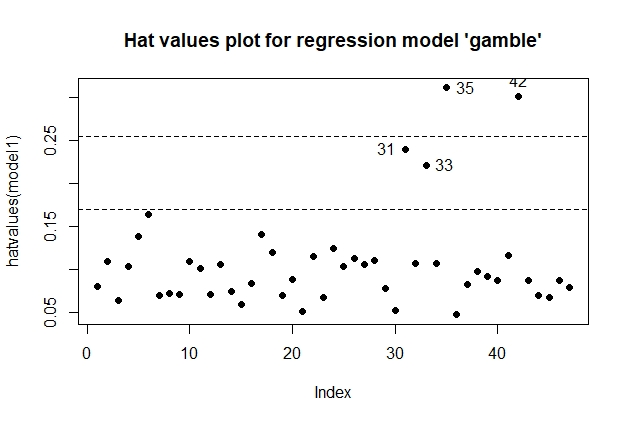
\includegraphics[width=.75\textwidth]{Hatvalue.JPEG}
	\caption{We identified four obervations (row number labeled) as large leverage points for they surpass our thresholds}
	\end{figure}
	
	\item Check for outliers by running an \texttt{outlierTest}. \vspace{.5cm}
	\vspace{.5cm}
	\lstinputlisting[language = R, firstline = 55, lastline = 61]{Alice-PS5.R}
	\newpage
	Output:
	\begin{Verbatim}
No Studentized residuals with Bonferroni p <
Largest |rstudent|:
rstudent unadjusted p-value Bonferroni p
24 6.016116         4.1041e-07   1.9289e-05
	\end{Verbatim}
	
	\begin{figure}[h!]\centering
	\label{Cook}
	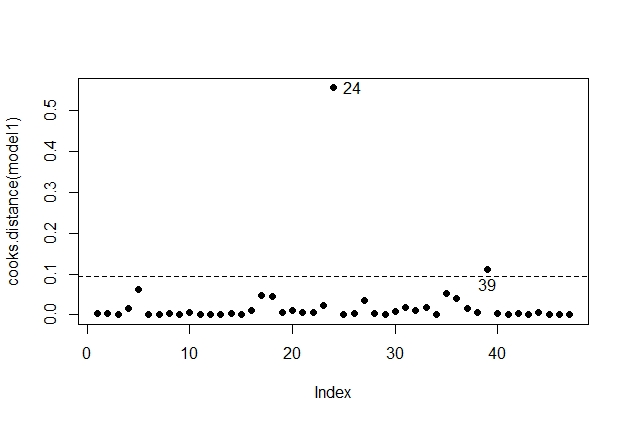
\includegraphics[width=.75\textwidth]{Outlier.JPEG}
	\caption{Plot of Cook's distance for regression model "gamble",     This suggest that the 24th observation in the dataset has the largest studentized residual and is a significant outlier $(P < 0.001)$}
	\end{figure}
	
    \vspace{1cm} 
	\item Check for influential points by creating a "Bubble plot" with the hat-values and studentized residuals.
	\lstinputlisting[language = R, firstline = 62, lastline = 69]{Alice-PS5.R}	
	
	\begin{figure}\centering
	\label{bubble}
	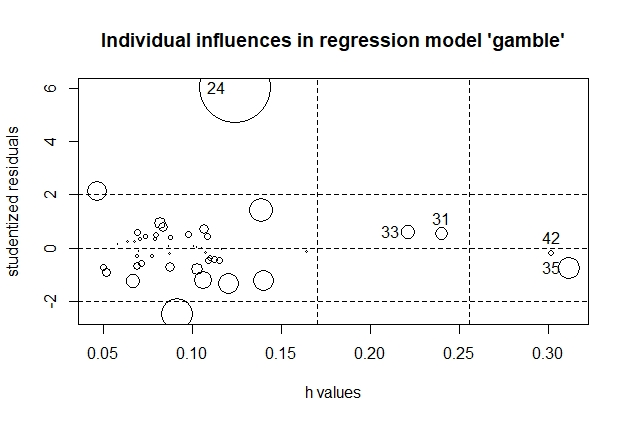
\includegraphics[width=\textwidth]{Bubble.JPEG}
	\caption{Bubble plot of influence measures for regression model "gamble". We can see the four large leverage points as well as the outlier "24", which has the biggest influence on the model}
	\end{figure}	
	% \item N/A.
\end{enumerate}

\end{document}
